\documentclass[tikz,border=5pt]{standalone}
% ============================================================
%  style.tex
%  Style commun pour les graphes de fonctions et d'intégrales
%  Usage : \input{style.tex}  (à placer après \documentclass)
% ============================================================

\usepackage{pgfplots}
\pgfplotsset{compat=1.18}
\usepackage[T1]{fontenc}
\usepackage{amsmath,amsfonts}
\usepackage{xcolor}
\usetikzlibrary{patterns}
\usepgfplotslibrary{fillbetween}

% ---- Couleurs standard ----
\colorlet{monGris}{black!45}   
\colorlet{monBleu}{blue!60}  

% ============================================================
%  Styles TikZ (\tikzset) : tout ce qui touche à l'apparence
%  (couleurs, épaisseurs, hachures, position des étiquettes...)
%  -> utilisables aussi bien sur \node, \draw, \addplot, etc.
% ============================================================
\tikzset{
  % Courbe "secondaire" en nuance de gris (tracé + étiquette)
  courbe/.style={thick},
  % Hachures
  hachure/.style={
    pattern=north east lines,
    pattern color=#1,
    draw=none,
    samples=100,
    /pgfplots/forget plot,
  },
  hachure/.default=black,
}

% ============================================================
%  Style pgfplots (\pgfplotsset) : options propres à l'environnement axis
%  (repère orthonormé, ticks, épaisseur des axes...)
%  -> ces clés n'existent que dans /pgfplots/, \tikzset ne peut pas les définir.
% ============================================================
\pgfplotsset{
    axes/.style={
    axis lines=middle,
    axis equal image,               % repère orthonormé
    thick,                          % épaisseur des axes et courbes
    samples=200,
  }
}


\begin{document}
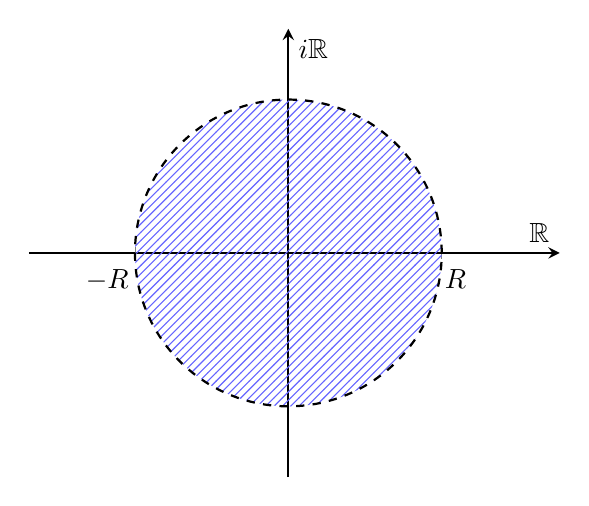
\begin{tikzpicture}
\begin{axis}[
    axes,
    xlabel={$\mathbb{R}$},
    ylabel={$i\mathbb{R}$},
    xmin=-4.4, xmax=4.6,
    ymin=-3.8, ymax=3.8,
    xticklabels={$R$},
    xtick={2.6},
    xticklabel style ={xshift=5pt},
    ytick=\empty,
    extra x ticks = {-2.6},
    extra x tick labels={$-R$},
    extra x tick style ={tick label style ={xshift=-15pt}},
    clip=false,
]

% Disque ouvert de convergence (rempli, frontière en pointillés)
\fill[pattern=north east lines, pattern color = monBleu] (axis cs:0,0) circle (2.6);
\draw[dashed, thick] (axis cs:0,0) circle (2.6);


% Comportement de la série
% \node[align=center, monBleu] at (axis cs:3,2.6) {convergence\\absolue};
% \node[align=center] at (axis cs:3.0,-2.6) {divergence\\grossière};

\end{axis}
\end{tikzpicture}
\end{document}
